\documentclass[10pt,twocolumn,letterpaper]{article}

\usepackage{cvpr}
\usepackage{times}
\usepackage{epsfig}
\usepackage{graphicx}
\usepackage{amsmath}
\usepackage{amssymb}
\usepackage{float}
\usepackage{listings}
%\usepackage{enumitem}

% Include other packages here, before hyperref.

% If you comment hyperref and then uncomment it, you should delete
% egpaper.aux before re-running latex.  (Or just hit 'q' on the first latex
% run, let it finish, and you should be clear).
\usepackage[breaklinks=true,bookmarks=false]{hyperref}

\cvprfinalcopy % *** Uncomment this line for the final submission

\def\cvprPaperID{****} % *** Enter the CVPR Paper ID here
\def\httilde{\mbox{\tt\raisebox{-.5ex}{\symbol{126}}}}

% Pages are numbered in submission mode, and unnumbered in camera-ready
%\ifcvprfinal\pagestyle{empty}\fi
\setcounter{page}{1}
\begin{document}

%%%%%%%%% TITLE
\title{Deep Reinforcement Learning Report}

\author{Jiankai Sun\\
Shanghai Jiao Tong University\\
800, Rd Dongchuan, Shanghai, China\\
{\tt\small jiankai@sjtu.edu.cn}
% For a paper whose authors are all at the same institution,
% omit the following lines up until the closing ``}''.
% Additional authors and addresses can be added with ``\and'',
% just like the second author.
% To save space, use either the email address or home page, not both
%\and
%Second Author\\
%Institution2\\
%First line of institution2 address\\
%{\tt\small secondauthor@i2.org}
}

\maketitle
%\thispagestyle{empty}

%%%%%%%%% ABSTRACT
\begin{abstract}
	In this paper, I make a summary of the Reinforcement Learning lessons given by David Silver. There is also some analysis of the codes \href{https://github.com/Kaixhin/Atari}{Atari} and \href{https://github.com/carpedm20/deep-rl-tensorflow}{TensorFlow implementation of Deep Reinforcement Learning papers}. 
%   The ABSTRACT is to be in fully-justified italicized text, at the top
%   of the left-hand column, below the author and affiliation
%   information. Use the word ``Abstract'' as the title, in 12-point
%   Times, boldface type, centered relative to the column, initially
%   capitalized. The abstract is to be in 10-point, single-spaced type.
%   Leave two blank lines after the Abstract, then begin the main text.
%   Look at previous CVPR abstracts to get a feel for style and length.
\end{abstract}

%%%%%%%%% BODY TEXT
\section{Introduction}

Reinforcement Learning includes Markov Decision Process(MDP), Planning by Dynamic Processes, Model-Free Prediction, Policy Gradient Method and so on. Persistent advantage learning, bootstrapped, dueling, double, deep recurrent, Q-network are implemented using Torch 7 in Atari project.
%Please follow the steps outlined below when submitting your manuscript to
%the IEEE Computer Society Press.  This style guide now has several
%important modifications (for example, you are no longer warned against the
%use of sticky tape to attach your artwork to the paper), so all authors
%should read this new version.

%-------------------------------------------------------------------------
\subsection{Markov Decision Process}

Major components of an RL Agent are Policy, Value Function and Model. A state $S_t$ is Markov if and only if
\begin{equation}
\mathbb{P}[S_{t+1}|S_t] = \mathbb{P}[S_{t+1}|S_1, ... , S_t]
\end{equation}
A future is independent of the past given the present. We use state transition matrix $P$ to define transition probabilities from all states $s$ to all successor states $s'$
\begin{equation}
P_{ss'}=\mathbb{P}[S_{t+1}=s'|S_t=s]
\end{equation}
A Markov Reward Process is a tuple $<S, A, P, R, \gamma>$
\begin{itemize}
	\item $S$ is a finite set of states
	\item $A$ is a finite set of actions
	\item $P$ is a state transition probability matrix,
		  $$P_{ss'}^{a} = \mathbb{P}[S_{t+1} = s'| S_t = s, A_t = a]$$
	\item R is a reward function, $$R_s^a = \mathbb{E}[R_{t+1}|S_t=s, A_t = a]$$
	\item $\gamma$ is a discount factor, $\gamma \in  [0, 1]$
\end{itemize}

Return $G_t$ $$G_t=\sum_{k=0}^{\infty} \gamma^k R_{t+k+1}$$

State value function $v_\pi (s)$
$$v_\pi (s) = \mathbb{E}_\pi [G_t|S_t = s]$$
Action value function $q_\pi (s, a)$
$$q_\pi (s, a) = \mathbb{E}_\pi [G_t|S_t = s, A_t = a]$$
Policy $\pi$ $$\pi (a|s) = \mathbb{P}[A_t = a|S_t=s]$$

There are also introductions about optimal function, Bellman expectation equation and Bellman optimal equation. Partially Observable Markov Decision Process is an MDP with hidden states.
\subsection{Planning by Dynamic Programming}

As for policy evaluation, there are iterative policy evaluation and improvement. 
As for value evaluation, A policy $\pi (a|s)$ achieves the optimal value from state s, $v_\pi (s) = v_\ast(s)$ (the principle of optimality), if and only if
\begin{itemize}
	\item For any state $s'$ reachable from $s$
	\item $\pi$ achieves the optimal value from state $s'$, $v_\pi (s') = v_\ast (s')$	 
\end{itemize}
Dynamic programming algorithms include asynchronous (in-place, prioritised sweeping, real-time) and synchronous. Extensions include full-width and sample backups. Approximate dynamic programming is used to approximate the value function.\\
Contraction Mapping Theorem:
For any metric space $V$ that is complete (i.e. closed) under an
operator $T(v)$, where $T$ is a $\gamma$-contraction,
\begin{itemize}
	\item $T$ converges to a unique fixed point
	\item At a linear convergence rate of 
$\gamma$
\end{itemize}
%By submitting a manuscript to CVPR, the authors guarantee that it has 
%not been previously published or accepted for publication in substantially 
%similar form in an archival peer-reviewed forum. Furthermore, no paper which 
%contains significant overlap with the contributions of this paper is neither 
%under review at the moment of submission nor will be submitted during the 
%CVPR 2014 review period to {\bf any of the following}: another conference,
%a workshop, or a journal. The authors also attest that they did not submit
%substantially similar submissions to CVPR 2014. {\bf Violation of any of
%these conditions will lead to rejection.} If you are not sure about the
%extent of overlap, you may upload a copy of the paper in question as
%supplementary material. Note that a Technical Report (departmental, 
%arXiv.org, etc.) that is put up without any form of direct peer-review is 
%{\bf NOT} considered a publication. Likewise, mention of the work under 
%review in a presentation is {\bf NOT} considered a violation.
%
%If there are papers that may appear to the reviewers
%to violate this condition, then it is your responsibility to: (1)~cite
%these papers (preserving anonymity as described in Section 1.6 below),
%(2)~argue in the body of your paper why your CVPR paper is non-trivially
%different from these concurrent submissions, and (3)~include anonymized
%versions of those papers in the supplemental material.

\subsection{Model-Free Prediction}

Temporal-Difference Learning can learn before knowing the final outcome. It can learn online after every step。 It can learn from incomplete sequences. It works in continuing (non-terminating) environments .However, TD has low variance, some bias and MC has high variance, zero bias. TD exploits Markov property while MC does not.\\
The sum of online updates is identical for forward-view and backward-view TD($\lambda$)
\begin{equation}
	\sum_{t=1}^{T}\alpha \delta_tE_t(s) = \sum_{t=1}^{T}\alpha (G_t^\lambda-V(S_t))1(S_t=s)
\end{equation}
%CVPR papers may be between 6 pages and 8 pages, with a \$100 per page added
%fee.  Overlength papers will simply not be reviewed.  This includes papers
%where the margins and formatting are deemed to have been significantly
%altered from those laid down by this style guide.  Note that this
%\LaTeX\ guide already sets figure captions and references in a smaller font.
%The reason such papers will not be reviewed is that there is no provision for
%supervised revisions of manuscripts.  The reviewing process cannot determine
%the suitability of the paper for presentation in eight pages if it is
%reviewed in eleven.  If you submit 8 for review expect to pay the added page
%charges for them. 

%-------------------------------------------------------------------------
\subsection{Model-Free Control}
\paragraph{On-policy Monte-Carlo Control} $\epsilon$-Greedy Policy improvement. \\
For any $\epsilon$-greedy policy, the $\epsilon$-greedy policy $\pi '$ with respect to $q\pi$ is an improvement, $v_{\pi '}(s) \geq v_{\pi}(s)$
\begin{equation}
\begin{aligned}
q_\pi (s, \pi '(s))&=\sum_{a \in A} \pi'(a|s) q_\pi (s,a)\\
&\geq \sum_{a \in A} \pi (a|s) q_\pi (s,a)\\
& = v_\pi (s)
\end{aligned}
\end{equation}
Greedy in the Limit with Infinite Exploration (GLIE) Monte-Carlo control converges to the optimal action-value function, $Q(s, a) \rightarrow q_\ast (s, a)$\\
Temporal-difference (TD) learning has several advantages over Monte-Carlo (MC), which including lower variance, online, incomplete sequences. State Action Reward State Action (SARSA) converges to the optimal action-value function, $Q(s, a) \rightarrow q_\ast (s, a)$, under the following conditions:
\begin{itemize}
	\item GLIE sequence of policies $\pi_t (a|s)$
	\item Robbins-Monro sequence of step-sizes $\alpha_t$
	$$\sum_{t=1}^{\infty}\alpha_t = \infty$$
	$$\sum_{t=1}^{\infty}\alpha_t^2 < \infty$$
\end{itemize}
\paragraph{Off-policy Learning} include importance sampling for Off-policy Monte-Carlo and for Off-policy TD. Q-Learning doesn't require importance sampling. Q-learning control converges to the optimal action-value function, $Q(s, a) \rightarrow q_\ast (s, a)$


%The \LaTeX\ style defines a printed ruler which should be present in the
%version submitted for review.  The ruler is provided in order that
%reviewers may comment on particular lines in the paper without
%circumlocution.  If you are preparing a document using a non-\LaTeX\
%document preparation system, please arrange for an equivalent ruler to
%appear on the final output pages.  The presence or absence of the ruler
%should not change the appearance of any other content on the page.  The
%camera ready copy should not contain a ruler. (\LaTeX\ users may uncomment
%the \verb'\cvprfinalcopy' command in the document preamble.)  Reviewers:
%note that the ruler measurements do not align well with lines in the paper
%--- this turns out to be very difficult to do well when the paper contains
%many figures and equations, and, when done, looks ugly.  Just use fractional
%references (e.g.\ this line is $095.5$), although in most cases one would
%expect that the approximate location will be adequate.

\subsection{Value Function Approximation}
To solve large problems, we can adopt value function approximation. In the part of incremental methods, the lecturer introduces gradient descent, linear function approximation, incremental prediction algorithm. As for Batch Reinforcement Learning, gradient descent is simple. But it is not sample efficient. Batch methods seek to find the best fitting value function. Least squares algorithms find parameter vector $w$ minimizing sum-squared error between $\hat{v}(s_t, w)$ and target values $v_t^\pi$. Deep Q-Networks uses experience replay and fixed Q-targets. Linear Least Squares Prediction Algorithms. Least Squares Policy Iteration Algorithm repeatedly re-evaluates experience $D$ with different policies.
%Please number all of your sections and displayed equations.  It is
%important for readers to be able to refer to any particular equation.  Just
%because you didn't refer to it in the text doesn't mean some future reader
%might not need to refer to it.  It is cumbersome to have to use
%circumlocutions like ``the equation second from the top of page 3 column
%1''.  (Note that the ruler will not be present in the final copy, so is not
%an alternative to equation numbers).  All authors will benefit from reading
%Mermin's description of how to write mathematics:
%\url{http://www.pamitc.org/documents/mermin.pdf}.
%
\subsection{Policy Gradient}
In Policy-Based Reinforcement Learning, a policy is generated directly from the value function. RL includes Value-Based RL and Policy-Based RL. In policy gradient, the score function is $\bigtriangledown_\theta log\pi_\theta(s,a)$. There are also Softmax Policy and Gaussian Policy. For any differentiable policy $\pi_\theta\theta(s, a)$, for any of the policy objective functions $J = J_1$; $J_{avR}$ ; or $\frac{1}{1-\gamma}$$J_{avV}$
the policy gradient is$$\bigtriangledown_\theta J(\theta)=\mathbb{E}_{\pi \theta}[\bigtriangledown_\theta log \pi_\theta(s, a)Q^{\pi_\theta}(s, a)]$$
The policy gradient has many equivalent forms: REINFORCE, Q Actor-Critic, Advantage Actor-Critic, TD Actor-Critic, TD($\lambda$) Actor-Critic, Natural Actor-Critic, Each leads a stochastic gradient ascent algorithm.
\subsection{Experiments}

I learned about several Github projects related to Reinforcement Learning shown as below. 


\begin{quote}
\begin{center}
    Atari\\
    \begin{quote}
    https://github.com/Kaixhin/Atari
    \end{quote}
    deep-rl-tensorflow
    
\end{center}

   TensorFlow implementation of Deep Reinforcement Learning papers.\\
   https://github.com/carpedm20/deep-rl-tensorflow
   
\end{quote}


\begin{quote}
\begin{center}
     DeepMind-Atari-Deep-Q-Learner
\end{center}
   The original code from the DeepMind article Human-level control through deep reinforcement learning

   https://github.com/kuz/DeepMind-Atari-Deep-Q-Learner
\end{quote}

\begin{quote}
	\begin{center}
		dqn
	\end{center}
	DQN implementation in Keras + TensorFlow + OpenAI Gym 
	
	https://github.com/tatsuyaokubo/dqn
\end{quote}
\subsubsection{Code Analysis}
Take the DQN implementation in Keras + TensorFlow + OpenAI Gym as an example, there are DQN and Double DQN implementation.
\paragraph{DQN}$\ $\\
Create q network
\begin{lstlisting}[frame=shadowbox]
self.s, self.q_values, 
q_network = self.build_network()
q_network_weights =
q_network.trainable_weights
\end{lstlisting}
Create target network
\begin{lstlisting}[frame=shadowbox]
self.st, self.target_q_values,
 target_network = self.build_network()
target_network_weights =
 target_network.trainable_weights
\end{lstlisting}
Define target network update operation
\begin{lstlisting}[frame=shadowbox]
self.update_target_network =
 [target_network_weights[i].
 assign(q_network_weights[i]) 
 for i in range
 (len(target_network_weights))]
\end{lstlisting}
Define loss and gradient update operation
\begin{lstlisting}[frame=shadowbox]
 self.a, self.y, self.loss,
  self.grads_update =  self.
  build_training_op(q_network_weights)
\end{lstlisting}
Initialize target network using tensorflow
\begin{lstlisting}[frame=shadowbox]
self.sess.run(self.update_target_network)
\end{lstlisting}
Initialize target network using tensorflow
\begin{lstlisting}[frame=shadowbox]
self.sess.run(self.update_target_network)
\end{lstlisting}
Function \emph{build\_network()} is defined using Keras, including three Convolution2D layers.
The first convolution layers include 32 convolution kernels, the size each convolution kernels 8 * 8. The second convolution layers include 64 convolution kernels, the size each convolution kernels $4 * 4$. The second convolution layers include 64 convolution kernels, the size each convolution kernels 3 * 3. Then, there is an all connection layer, to flatten the output of the last layer from two-dimensional to one dimension. Dense is a hidden layer. $s$ is a placeholder.\\
Function \emph{build\_training\_op()} contains two placeholders $a,y$. Use $tf.one\_hot$ and $tf.reduced\_sum$ to convert action to one hot vector. $tf.reduce\_mean$ is utilized to computes the mean of elements across dimensions of a tensor. $tf.train.RMSPropOptimizer$ is an optimizer that implements the RMSProp algorithm.\\
Function \emph{get\_initial\_state, run} and \emph{get\_action} are implemented with the help of numpy. Module \emph{random.random()} is imported to generate random number. Anneal epsilon linearly over time. Function \emph{run} first, clips all positive rewards at 1 and all negative rewards at -1, leaving 0 rewards unchanged, then, store transition in replay memory. Start to train the network, update target network and save network.\\
Function \emph{train\_network()} establishes a sample random minibatch of transition from replay memory first. Then calculate the loss through tensorflow. Other functions include \emph{setup\_summary(), load\_network, preprocess and get\_action\_at\_test }. In the \emph{main()}, using gym.make to build the environment. There are two modes: train mode and test mode.
\paragraph{Double DQN}
In class \emph{Agent}, there are also replay memory, q network, target network, update operation (including target network and loss and gradient). The difference is in function \emph{train\_network()}
\begin{lstlisting}[title=dqn.py, frame=shadowbox]
target_q_values_batch =
 self.target_q_values.eval(feed_dict=
 {self.st: np.float32(np.array
 (next_state_batch) / 255.0)})
y_batch = reward_batch + (1 - 
terminal_batch) * GAMMA * 
np.max(target_q_values_batch, axis=1)
\end{lstlisting}

\begin{lstlisting}[title=ddqn.py, frame=shadowbox]
next_action_batch =
 np.argmax(self.q_values.eval(feed_dict
 ={self.s: next_state_batch}), axis=1)
target_q_values_batch =
 self.target_q_values.eval(feed_dict
 ={self.st: next_state_batch})
for i in xrange(len(minibatch)):
y_batch.append(reward_batch[i] +
 (1 - terminal_batch[i]) * GAMMA *
  target_q_values_batch[i]
  [next_action_batch[i]])
\end{lstlisting}
 
\subsubsection{The Training Process}
By using AWS EC2 p2 instance, I try to train Atari and DeepMind-Atari-Deep-Q-Learner on the platform. As for deep-rl-tensorflow, there is a fatal error I will solve later.
\begin{figure}[H]
	\begin{center}
		%\fbox{\rule{0pt}{2in} \rule{0.9\linewidth}{0pt}}
		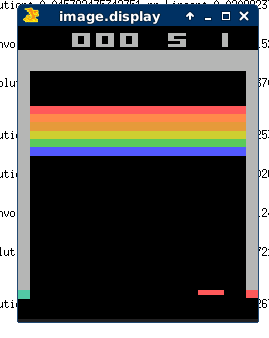
\includegraphics[width=0.8\linewidth]{img/fig1.png}
	\end{center}
	\caption{Snapshot of training  DeepMind-Atari-Deep-Q-Learner}
	\label{fig:long}
	\label{fig:onecol}
\end{figure}

\begin{figure}[H]
	\begin{center}
		%\fbox{\rule{0pt}{2in} \rule{0.9\linewidth}{0pt}}
		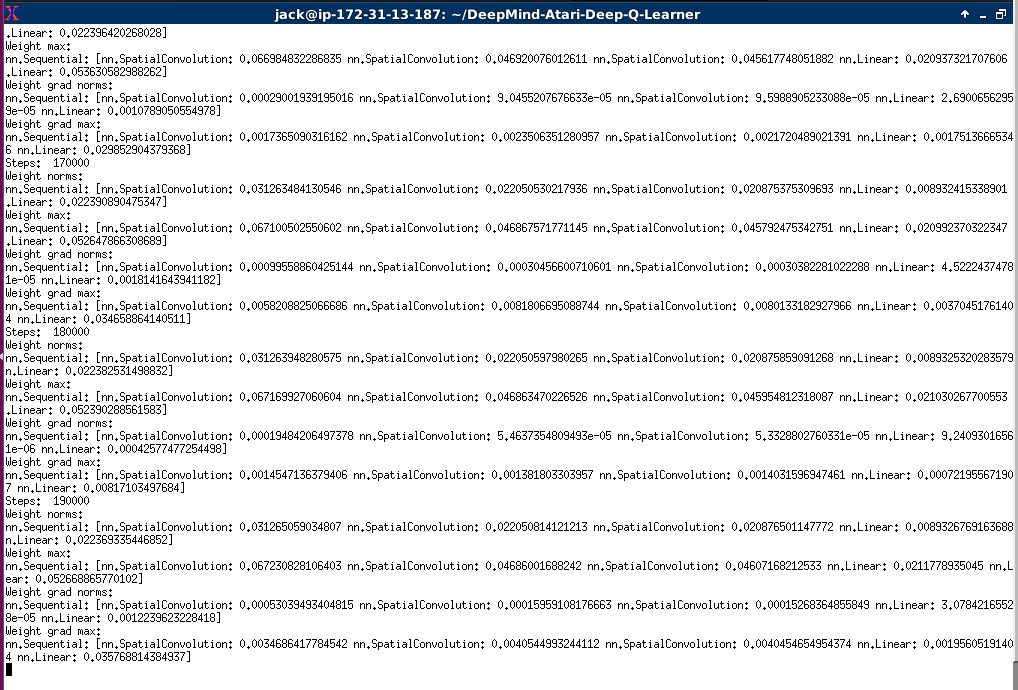
\includegraphics[width=0.8\linewidth]{img/fig2.png}
	\end{center}
	\caption{Snapshot of iteration}
	\label{fig:long}
	\label{fig:onecol}
\end{figure}
\begin{figure}[H]
	\begin{center}
		%\fbox{\rule{0pt}{2in} \rule{0.9\linewidth}{0pt}}
		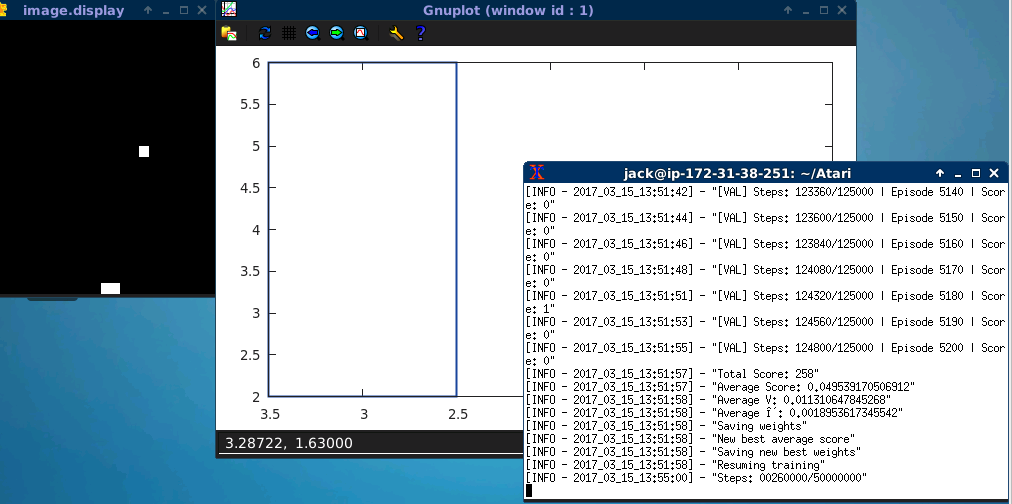
\includegraphics[width=0.8\linewidth]{img/fig3.png}
	\end{center}
	\caption{Snapshot of training  Atari}
	\label{fig:long}
	\label{fig:onecol}
\end{figure}


%If you are making a submission to another conference at the same time,
%which covers similar or overlapping material, you may need to refer to that
%submission in order to explain the differences, just as you would if you
%had previously published related work.  In such cases, include the
%anonymized parallel submission~\cite{Authors14} as additional material and
%cite it as
\begin{quote}
[1] Authors. ``The frobnicatable foo filter'', F\&G 2014 Submission ID 324,
Supplied as additional material {\tt fg324.pdf}.
\end{quote}

Finally, you may feel you need to tell the reader that more details can be
found elsewhere, and refer them to a technical report.  For conference
submissions, the paper must stand on its own, and not {\em require} the
reviewer to go to a techreport for further details.  Thus, you may say in
the body of the paper ``further details may be found
in~\cite{Authors14b}''.  Then submit the techreport as additional material.
Again, you may not assume the reviewers will read this material.

Sometimes your paper is about a problem which you tested using a tool which
is widely known to be restricted to a single institution.  For example,
let's say it's 1969, you have solved a key problem on the Apollo lander,
and you believe that the CVPR70 audience would like to hear about your
solution.  The work is a development of your celebrated 1968 paper entitled
``Zero-g frobnication: How being the only people in the world with access to
the Apollo lander source code makes us a wow at parties'', by Zeus \etal.

You can handle this paper like any other.  Don't write ``We show how to
improve our previous work [Anonymous, 1968].  This time we tested the
algorithm on a lunar lander [name of lander removed for blind review]''.
That would be silly, and would immediately identify the authors. Instead
write the following:
\begin{quotation}
\noindent
   We describe a system for zero-g frobnication.  This
   system is new because it handles the following cases:
   A, B.  Previous systems [Zeus et al. 1968] didn't
   handle case B properly.  Ours handles it by including
   a foo term in the bar integral.

   ...

   The proposed system was integrated with the Apollo
   lunar lander, and went all the way to the moon, don't
   you know.  It displayed the following behaviours
   which show how well we solved cases A and B: ...
\end{quotation}
As you can see, the above text follows standard scientific convention,
reads better than the first version, and does not explicitly name you as
the authors.  A reviewer might think it likely that the new paper was
written by Zeus \etal, but cannot make any decision based on that guess.
He or she would have to be sure that no other authors could have been
contracted to solve problem B.

FAQ: Are acknowledgements OK?  No.  Leave them for the final copy.


\begin{figure}[t]
\begin{center}
\fbox{\rule{0pt}{2in} \rule{0.9\linewidth}{0pt}}
   %\includegraphics[width=0.8\linewidth]{egfigure.eps}
\end{center}
   \caption{Example of caption.  It is set in Roman so that mathematics
   (always set in Roman: $B \sin A = A \sin B$) may be included without an
   ugly clash.}
\label{fig:long}
\label{fig:onecol}
\end{figure}

\subsection{Miscellaneous}

\noindent
Compare the following:\\
\begin{tabular}{ll}
 \verb'$conf_a$' &  $conf_a$ \\
 \verb'$\mathit{conf}_a$' & $\mathit{conf}_a$
\end{tabular}\\
See The \TeX book, p165.

The space after \eg, meaning ``for example'', should not be a
sentence-ending space. So \eg is correct, {\em e.g.} is not.  The provided
\verb'\eg' macro takes care of this.

When citing a multi-author paper, you may save space by using ``et alia'',
shortened to ``\etal'' (not ``{\em et.\ al.}'' as ``{\em et}'' is a complete word.)
However, use it only when there are three or more authors.  Thus, the
following is correct: ``
   Frobnication has been trendy lately.
   It was introduced by Alpher~\cite{Alpher02}, and subsequently developed by
   Alpher and Fotheringham-Smythe~\cite{Alpher03}, and Alpher \etal~\cite{Alpher04}.''

This is incorrect: ``... subsequently developed by Alpher \etal~\cite{Alpher03} ...''
because reference~\cite{Alpher03} has just two authors.  If you use the
\verb'\etal' macro provided, then you need not worry about double periods
when used at the end of a sentence as in Alpher \etal.

For this citation style, keep multiple citations in numerical (not
chronological) order, so prefer \cite{Alpher03,Alpher02,Authors14} to
\cite{Alpher02,Alpher03,Authors14}.


\begin{figure*}
\begin{center}
\fbox{\rule{0pt}{2in} \rule{.9\linewidth}{0pt}}
\end{center}
   \caption{Example of a short caption, which should be centered.}
\label{fig:short}
\end{figure*}

%------------------------------------------------------------------------
\section{Formatting your paper}

All text must be in a two-column format. The total allowable width of the
text area is $6\frac78$ inches (17.5 cm) wide by $8\frac78$ inches (22.54
cm) high. Columns are to be $3\frac14$ inches (8.25 cm) wide, with a
$\frac{5}{16}$ inch (0.8 cm) space between them. The main title (on the
first page) should begin 1.0 inch (2.54 cm) from the top edge of the
page. The second and following pages should begin 1.0 inch (2.54 cm) from
the top edge. On all pages, the bottom margin should be 1-1/8 inches (2.86
cm) from the bottom edge of the page for $8.5 \times 11$-inch paper; for A4
paper, approximately 1-5/8 inches (4.13 cm) from the bottom edge of the
page.

%-------------------------------------------------------------------------
\subsection{Margins and page numbering}

All printed material, including text, illustrations, and charts, must be kept
within a print area 6-7/8 inches (17.5 cm) wide by 8-7/8 inches (22.54 cm)
high.
Page numbers should be in footer with page numbers, centered and .75
inches from the bottom of the page and make it start at the correct page
number rather than the 4321 in the example.  To do this fine the line (around
line 23)  
\begin{verbatim}
%\ifcvprfinal\pagestyle{empty}\fi
\setcounter{page}{4321}
\end{verbatim}
where the number 4321 is your assigned starting page.  

Make sure the first page is numbered by commenting out the first page being
empty on line 46
\begin{verbatim}
%\thispagestyle{empty}
\end{verbatim}


%-------------------------------------------------------------------------
\subsection{Type-style and fonts}

Wherever Times is specified, Times Roman may also be used. If neither is
available on your word processor, please use the font closest in
appearance to Times to which you have access.

MAIN TITLE. Center the title 1-3/8 inches (3.49 cm) from the top edge of
the first page. The title should be in Times 14-point, boldface type.
Capitalize the first letter of nouns, pronouns, verbs, adjectives, and
adverbs; do not capitalize articles, coordinate conjunctions, or
prepositions (unless the title begins with such a word). Leave two blank
lines after the title.

AUTHOR NAME(s) and AFFILIATION(s) are to be centered beneath the title
and printed in Times 12-point, non-boldface type. This information is to
be followed by two blank lines.

The ABSTRACT and MAIN TEXT are to be in a two-column format.

MAIN TEXT. Type main text in 10-point Times, single-spaced. Do NOT use
double-spacing. All paragraphs should be indented 1 pica (approx. 1/6
inch or 0.422 cm). Make sure your text is fully justified---that is,
flush left and flush right. Please do not place any additional blank
lines between paragraphs.

Figure and table captions should be 9-point Roman type as in
Figures~\ref{fig:onecol} and~\ref{fig:short}.  Short captions should be centred.

\noindent Callouts should be 9-point Helvetica, non-boldface type.
Initially capitalize only the first word of section titles and first-,
second-, and third-order headings.

FIRST-ORDER HEADINGS. (For example, {\large \bf 1. Introduction})
should be Times 12-point boldface, initially capitalized, flush left,
with one blank line before, and one blank line after.

SECOND-ORDER HEADINGS. (For example, { \bf 1.1. Database elements})
should be Times 11-point boldface, initially capitalized, flush left,
with one blank line before, and one after. If you require a third-order
heading (we discourage it), use 10-point Times, boldface, initially
capitalized, flush left, preceded by one blank line, followed by a period
and your text on the same line.

%-------------------------------------------------------------------------
\subsection{Footnotes}

Please use footnotes\footnote {This is what a footnote looks like.  It
often distracts the reader from the main flow of the argument.} sparingly.
Indeed, try to avoid footnotes altogether and include necessary peripheral
observations in
the text (within parentheses, if you prefer, as in this sentence).  If you
wish to use a footnote, place it at the bottom of the column on the page on
which it is referenced. Use Times 8-point type, single-spaced.


%-------------------------------------------------------------------------
\subsection{References}

List and number all bibliographical references in 9-point Times,
single-spaced, at the end of your paper. When referenced in the text,
enclose the citation number in square brackets, for
example~\cite{Authors14}.  Where appropriate, include the name(s) of
editors of referenced books.

\begin{table}
\begin{center}
\begin{tabular}{|l|c|}
\hline
Method & Frobnability \\
\hline\hline
Theirs & Frumpy \\
Yours & Frobbly \\
Ours & Makes one's heart Frob\\
\hline
\end{tabular}
\end{center}
\caption{Results.   Ours is better.}
\end{table}

%-------------------------------------------------------------------------
\subsection{Illustrations, graphs, and photographs}

All graphics should be centered.  Please ensure that any point you wish to
make is resolvable in a printed copy of the paper.  Resize fonts in figures
to match the font in the body text, and choose line widths which render
effectively in print.  Many readers (and reviewers), even of an electronic
copy, will choose to print your paper in order to read it.  You cannot
insist that they do otherwise, and therefore must not assume that they can
zoom in to see tiny details on a graphic.

When placing figures in \LaTeX, it's almost always best to use
\verb+\includegraphics+, and to specify the  figure width as a multiple of
the line width as in the example below
{\small\begin{verbatim}
   \usepackage[dvips]{graphicx} ...
   \includegraphics[width=0.8\linewidth]
                   {myfile.eps}
\end{verbatim}
}


%-------------------------------------------------------------------------
\subsection{Color}

Color is valuable, and will be visible to readers of the electronic copy.
However ensure that, when printed on a monochrome printer, no important
information is lost by the conversion to grayscale.

%------------------------------------------------------------------------
\section{Final copy}

You must include your signed IEEE copyright release form when you submit
your finished paper. We MUST have this form before your paper can be
published in the proceedings.


{\small
\bibliographystyle{ieee}
\bibliography{egbib}
}

\end{document}
